\section{Solution Development}

The solution development for the project was a process that involved several stages that were established over time. Thus, the solution was adapted according to new requirements. The development involved not only software but also hardware components, which made the protocol development in a laboratory environment essential to ensure system effectiveness. Since part of the development was carried out outside the laboratory, a component that simulates the implemented hardware was also developed. The solution took into account not only its usability, but also the difficulties and limitations encountered during the development process.

\subsection{Requirements}

This section will identify all functional and non-functional requirements established throughout the internship:

\begin{itemize}
    \item[] Functional requirements:
        \begin{itemize}
            \item Temperature data reading: The intern must develop a temperature data reading system; 
            \item Graphical interface: The solution must include a graphical interface that will allow the user to control the test;
            \item Real-time visualization of obtained data: the developed system must allow the user to visualize the test data obtained in real time;
            \item Database: All values obtained from the test must be stored in a local database;
            \item Communication: The system must ensure communication between devices (between the RPI and the EVSE and between the RPI and the MainPC).
        \end{itemize}
    \item[] Non-functional requirements:
        \begin{itemize}
            \item Performance: The system must be capable of processing data in real time without significant delays;
            \item Scalability: The system must be capable of supporting an increase in data volume without compromising performance;
            \item Reliability: The system must ensure data integrity and availability during operation;
            \item Security: The system must ensure minimum data security standards and protection against unauthorized access;
            \item Maintainability: The system must be designed to facilitate maintenance and updates over time.
        \end{itemize}
    \item[] Constraints:
        \begin{itemize}
            \item The entire developed system must be limited to the material and resources available in the laboratory;
            \item The system must be tested in a laboratory environment to ensure result fidelity;
            \item The system must be capable of operating in different environments without losing its functionality.
        \end{itemize}
\end{itemize}

\subsection{Architecture and technologies}

Throughout the internship, numerous technologies and architectures were considered to meet the client's requirements. As the requirements changed throughout the project, the project structure ended up being adjusted. This section will address the different architectures and technologies approached and their reasons for being selected.

\subsubsection{Hardware components}
The hardware components used were limited to the availability of resources and materials in the laboratory. For the solution implementation, a Raspberry Pi 3 and 4 DS18B20 sensors were used.

For protocol validation, an EVSE charger developed by the Laboratory and a thermal chamber (incubator) IMP 400 from HERATERM (available in the Laboratory) were used.

The Raspberry Pi 3 is a low-cost and highly versatile microcomputer, ideal for prototyping and automation projects. Another advantage is its ability to connect to various devices and sensors, facilitating integration in IoT projects. The Raspbian operating system was installed on the RPI, which provides a user-friendly interface and support for various libraries necessary for project development, namely a set of drivers and configurations to use the Raspberry's GPIO input. The GPIO input was essential for communication between the DS18B20 sensors and the Raspberry Pi, allowing reading and control of connected devices. Another advantage of the Raspberry is the integration of a network card in the system, which facilitated communication with other devices and data exchange between them. For all configuration and establishment of communication between devices, the book \cite{Molloy_2016} was used.

The DS18B20 sensors are used to measure temperature and are connected to the Raspberry Pi through the GPIO input, allowing precise reading of temperature data. This sensor was selected for the following reasons:
\begin{itemize}
    \item Versatility: The sensor has a long wire which helps in positioning the sensors inside the thermal chamber. Additionally, the sensor is encapsulated, making it resistant to adverse environments.
    \item Digital temperature reading: The RPI's GPIO input only reads digital values and not analog values (very common in temperature sensors). The DS18B20 sensor reads temperature digitally, which facilitates data acquisition (does not require an analog module).
    \item Cost: The sensors are affordable and available in the market.
\end{itemize}

The EVSE charger developed by INESCTEC is an AC (alternating current) charger, single-phase (230VAC), with a nominal power of 7.4kW ~= 32A, which has various installed sensors that allow measuring current, voltage, frequency, and temperature values (temperature values refer to the circuit). By reading voltage and current, power can be calculated and power consumption (W) over time gives us consumption or charging in energy (W/h), which is essential to see the efficiency of electric car charging over time. Inside the charger there is a Raspberry Pi that manages charging control and enables EVSE communication with an INESC database for sending charging data.

The IMP 400 is a thermal chamber that allows controlling the internal temperature, ensuring controlled conditions for conducting tests. It has the capacity to maintain constant internal temperature between 5°C and 70°C (which covers the temperature range experienced in Portugal). Internally it has a temperature sensor that allows knowing the chamber temperature during the test. Finally, the thermal chamber also has an RS 232 input that allows serial port communication with the Raspberry Pi. Due to a limitation of the thermal chamber itself, only query commands are available (allows, for example, obtaining the temperature of the chamber's internal sensor), but set commands (for example, changing the chamber temperature) are not available. For better understanding of the thermal chamber functionalities, its manual \cite{chamber_manual} was used and for more specific questions, the HERATERM support team.

Additionally, other components such as resistors, cables, and connectors were also used to ensure communication between the devices and the Raspberry Pi.

\subsubsection{Software components}

The software components used were the main targets in the study of architectures and technologies. The developed system consists of a set of modules that work together to ensure system functionality. The main software components used were: 
\begin{itemize}
    \item[.] Operating System: The operating system used on the RPI was Raspbian, which is a Linux distribution optimized for the Raspberry Pi. Raspbian provides a user-friendly interface and support for various libraries necessary for project development;
    \item[.] Programming Language: The programming language used was Python, which is widely used in automation and IoT projects due to its simplicity and versatility. Python has various libraries that facilitate communication with sensors and manipulation of obtained data;
    \item[.] Database: To store data obtained from sensors, MySQL was used, which is a widely used relational database management system. MySQL was chosen due to its robustness, scalability, and ease of use, in addition to being compatible with Python through the MySQL Connector library. Another important factor is that it is the main database system used in the laboratory, which facilitated integration with other existing systems;
    \item[.] Graphical Interface: To create the system's graphical interface, the PyQt library was used, which is a graphical interface development library for Python;
    \item[.] Dashboard: For real-time visualization of obtained data, Grafana was used, an open-source data visualization platform that allows creating interactive and customized dashboards;
    \item[.] Bootstrapping: To ensure correct system initialization, Ansible was used for installation and configuration of necessary software components on the RPI and dockerfile with devcontainer integration on the MainPC.
\end{itemize}

In addition to these components, other software was used that helped in protocol development, namely:
\begin{itemize}
    \item[.] Git: For source code version control and to facilitate file transfer from the development computer to the RPI;
    \item[.] Visual Studio Code: As IDE for source code development;
    \item[.] MySQL Workbench: For MySQL database management, allowing creation and manipulation of tables, queries, and other database objects;
    \item[.] RealVNC: For remote access to the Raspberry Pi, allowing visualization and control of the system's graphical interface from another computer;
    \item[.] Drawio and Mermaid: For creating diagrams that help visualize system architecture and project planning;
    \item[.] Fritzing: Electronic prototyping software that was used to draw the DS18B20 sensors connection circuit to the Raspberry Pi, facilitating circuit understanding and implementation.
\end{itemize}

\subsection{Developed solution}

A temperature test corresponds to a process of obtaining temperature data over a period of time that can present characteristics such as the initial temperature of the thermal chamber and its final temperature. The protocol's main objective is to ensure the necessary conditions for conducting the temperature test, in addition to considering other factors such as communication between devices, sensor data reading, and visualization of obtained data.

To help interpret the test data obtained, Mean Absolute Error (MAE) and Root Mean Square Error (RMSE) were used to calculate the moment when the temperature read by the thermal chamber control sensor and the control sensor stabilized.

The developed solution can be divided into two main components: 
\begin{itemize}
    \item[.] \textbf{RPI}: Corresponds to the part of the system that is responsible for controlling the DS18B20 temperature sensors, obtaining temperature data from the thermal chamber and EVSE, and communicating with the MainPC about the test status;
    \item[.] \textbf{MainPC}: Corresponds to the part of the system that is responsible for serving as a user interface through a graphical interface. Additionally, it is responsible for communicating with the RPI about actions to be performed, such as starting or stopping the test. It is on the MainPC that a dashboard (Grafana) is installed that allows visualizing obtained data in real time and a database (MySQL) that stores test data.
\end{itemize} 

Both components have a MySQL database that stores test data, allowing subsequent data consultation and analysis. The schema of both databases is the same. To be able to see results obtained in real time, both components have a data migration system through scheduling. For this to be possible, communication between the RPI and MainPC is essential.

All subsystems are integrated with parallelism via threads, which allows different system components to function independently and simultaneously, in addition to being easy to deactivate via .env. On the MainPC, signals are also used (via pyqtSignal) for the graphical interface thread to communicate with the other MainPC threads. 

Thus, the protocol scheme can be translated into the following diagram:
\begin{figure}[H]
    \centering
    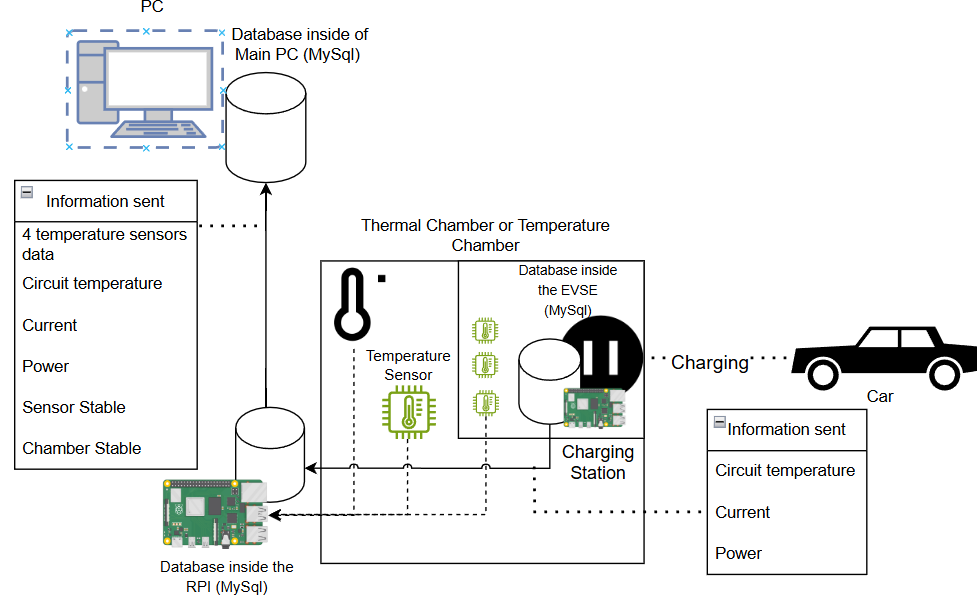
\includegraphics[width=0.8\textwidth]{figures/protocol_diagram.png}
    \caption{Communication protocol diagram between RPI and MainPC}
    \label{fig:diagrama_protocolo}
\end{figure}

In the following sections, the different essential system components will be addressed, as well as their installation.

Another important point to consider is that the system is modular, which allows easily disabling features, changing configurations (IPs, ports, etc.), and modifying parameters. For this, .env files were used that allow defining system environment variables, facilitating configuration. More information can be found in the general protocol documentation [DOCUMENTATION].

\subsubsection{DS18B20 temperature sensors and circuit}

For reading temperature data from DS18B20 sensors, a circuit was developed that allows connecting the sensors to the Raspberry Pi through the GPIO input. Since the circuit can be soldered, it allows greater robustness and reliability in sensor connections.

\begin{figure}[H]
    \centering
    \begin{minipage}{0.6\textwidth}
        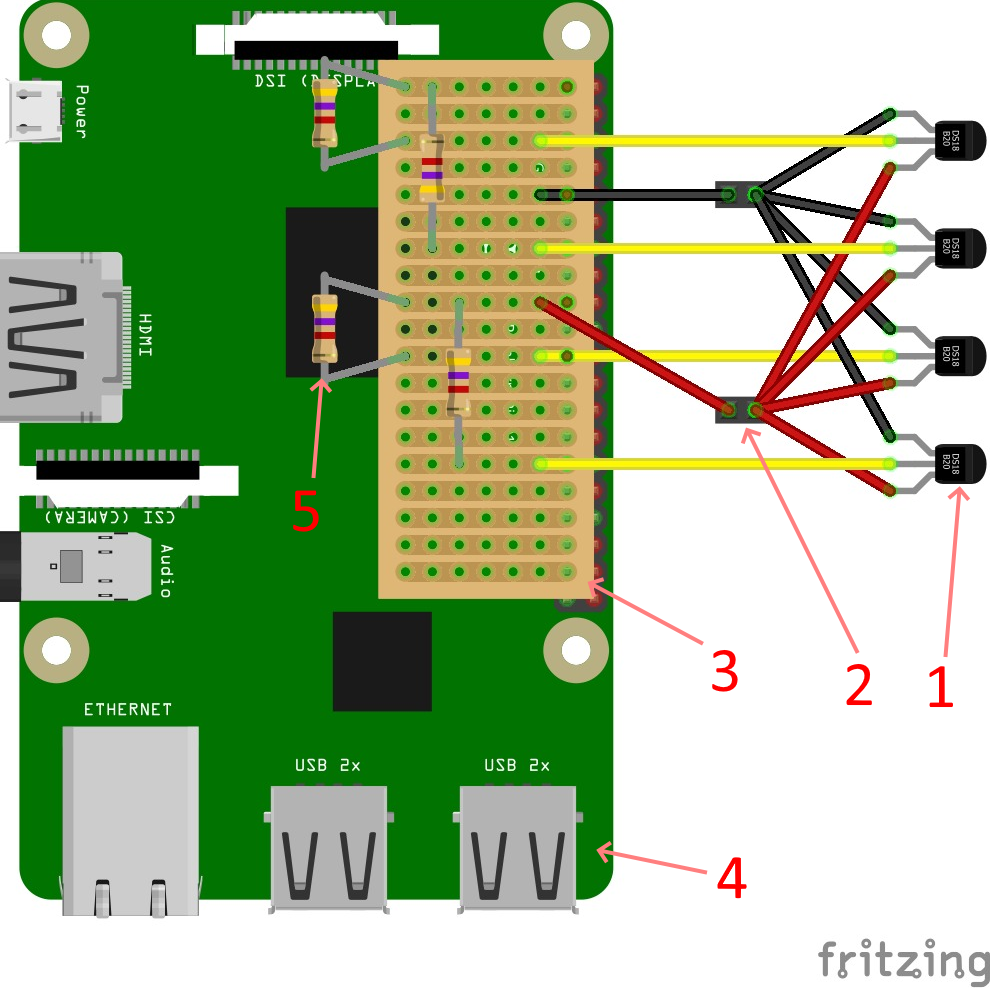
\includegraphics[width=\linewidth]{figures/circuit_dig.png}
    \end{minipage}%
    \hfill
    \begin{minipage}{0.35\textwidth}
        \small
        \textbf{Legend:}
        \begin{enumerate}
            \item DS18B20 Sensor 
            \item Connector
            \item Connection busboard
            \item RPI
            \item $4.7\,\mathrm{k}\Omega$ resistor
        \end{enumerate}
    \end{minipage}
    \caption{DS18B20 sensors connection circuit diagram to RPI}
    \label{fig:circuit_dig}
\end{figure}

\begin{figure}[H]
    \centering
    \begin{minipage}{0.48\textwidth}
        \centering
        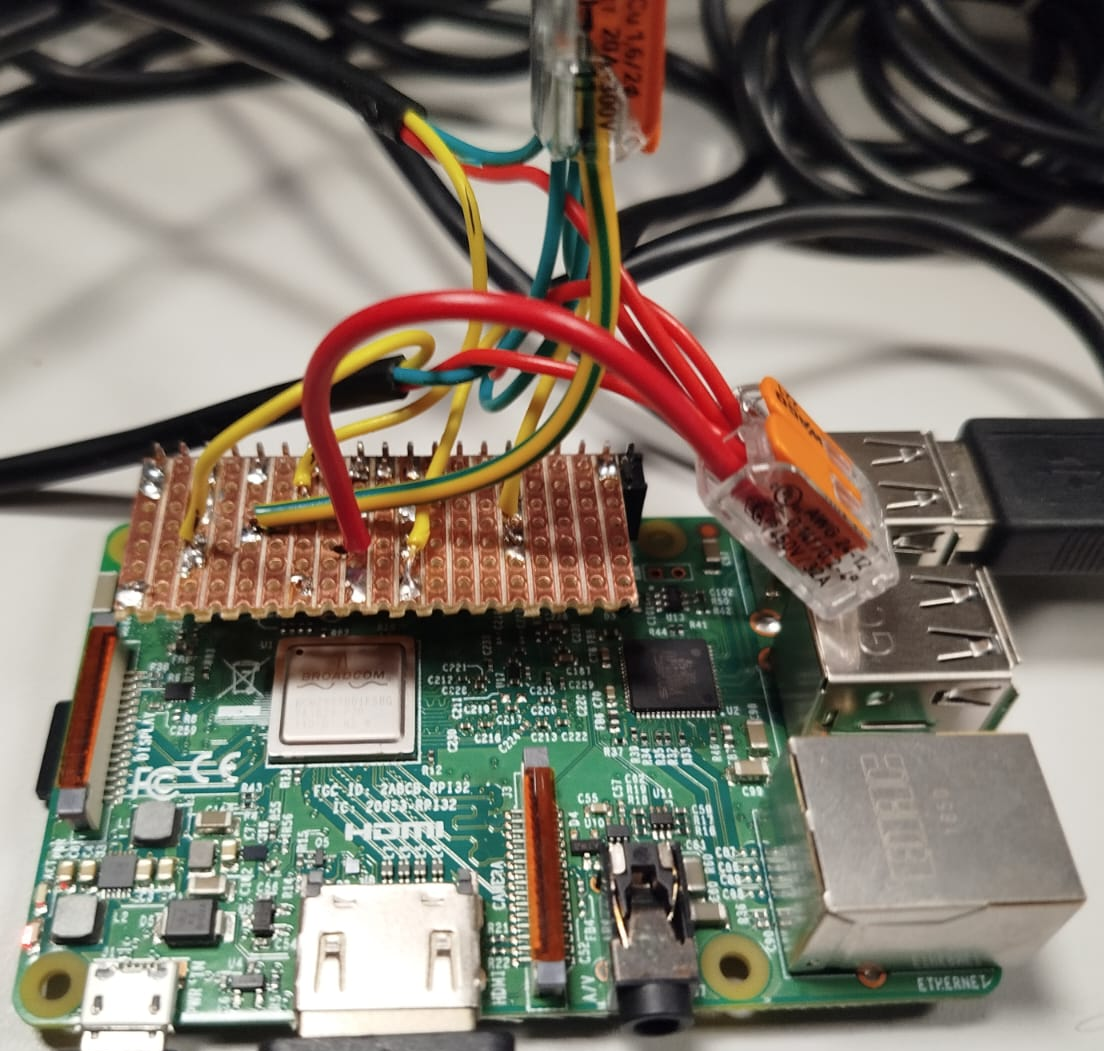
\includegraphics[width=\linewidth]{figures/circuit_1.png}
        \caption{Top view of DS18B20 sensors connection circuit to RPI}
        \label{fig:circuit_1}
    \end{minipage}\hfill
    \begin{minipage}{0.48\textwidth}
        \centering
        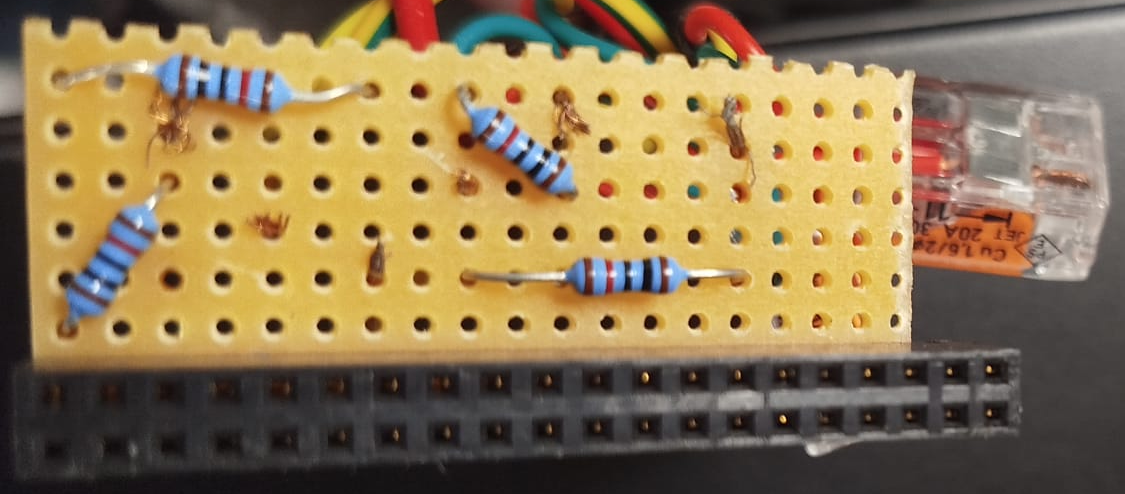
\includegraphics[width=\linewidth]{figures/circuit_2.png}
        \caption{Resistors view of DS18B20 sensors connection circuit to RPI}
        \label{fig:circuit_2}
    \end{minipage}
\end{figure}

This circuit allows connection of more sensors, however we decided to install only 4 DS18B20 sensors, one of the sensors is used to measure the thermal chamber temperature (serving as chamber temperature control) and the other three are positioned inside the EVSE at different locations to measure the charger temperature at different points.

For its hardware and software implementation (sensor reading), the sites \cite{Brian_Mark_Benoit_Santos_Alessandro_2023} and \cite{Campbell_2025}, and the DS18B20 sensor datasheet \cite{ds_datasheet} were used.

\subsubsection{Graphical interface}

The graphical interface was developed using the PyQt library and has as its main objective to help the user control the temperature test, allowing to create (establish time, test temperature and test description), start the temperature test, forcibly stop the test, and extend the test duration. The interface was developed to be easy to implement other functionalities in the future.

\begin{figure}[H]
    \centering
    \begin{minipage}{0.6\textwidth}
        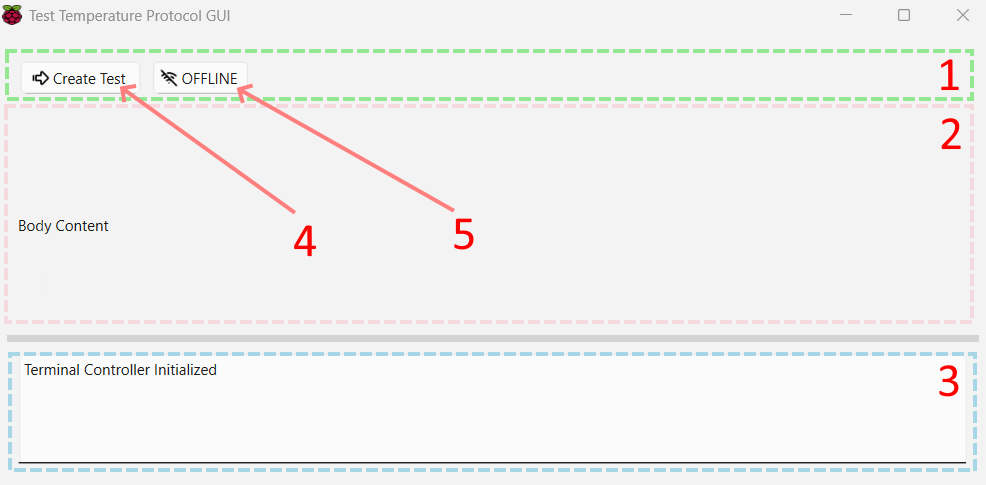
\includegraphics[width=\linewidth]{figures/gui_1.png}
    \end{minipage}%
    \hfill
    \begin{minipage}{0.35\textwidth}
        \small
        \textbf{Legend:}
        \begin{enumerate}
            \item Upbar
            \item Body
            \item Terminal
            \item Create a Test button
            \item RPI connection button
        \end{enumerate}
    \end{minipage}
    \caption{Protocol graphical interface}
    \label{fig:gui_1}
\end{figure}

The Connection button allows the user to establish connection with the RPI (with IP and port parameters defined in the .env file). After the connection is established, the user can create a temperature test through the Create a Test button, with the window appearing as a pop-up.

\begin{figure}[H]
    \centering
    \begin{minipage}{0.6\textwidth}
        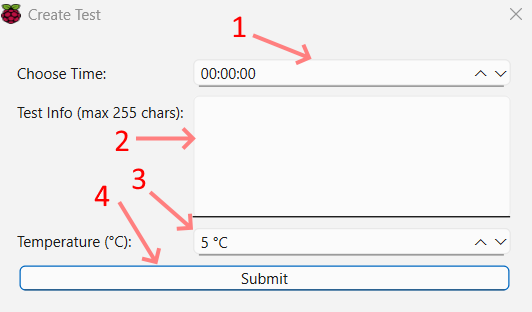
\includegraphics[width=\linewidth]{figures/gui_2.png}
    \end{minipage}%
    \hfill
    \begin{minipage}{0.35\textwidth}
        \small
        \textbf{Legend:}
        \begin{enumerate}
            \item Test timer
            \item Test description
            \item Test temperature
            \item Test submission button
        \end{enumerate}
    \end{minipage}
    \caption{Temperature test creation pop-up}
    \label{fig:gui_2}
\end{figure}

If the form is filled correctly (test time is greater than 0), the test is created and communicated to the RPI (DS18B20 sensors). More information about the communication process in \autoref{sec:comunicacao}.

To communicate user interactions with other MainPC threads (communication and scheduling), pyqtSignal (native to PyQt) was used, which allows sending signals between different MainPC threads.

\subsubsection{Communication}     \label{sec:comunicacao}

Communication between the two devices is essential for creating/controlling temperature tests, but also as the main way to maintain synchronization of the scheduling system of the two devices (MainPC and RPI). It also helps to notify the MainPC scheduling system when the control sensor and thermal chamber sensor have stabilized.

Communication between the RPI and MainPC is done through an SSL/TLS protocol to ensure the security of transmitted data. For this, there is a need to create an SSL/TLS certificate that is used to establish the secure connection between the two devices.

Although communication works peer to peer, to facilitate implementation the RPI behaves as a server (opens a port where it waits for a connection) and the MainPC as a client (connects to the RPI). After the connection is established and certificate authentication is validated, the RPI does not accept any more connections, establishing a peer-to-peer system.

\begin{figure}[H]
    \centering
    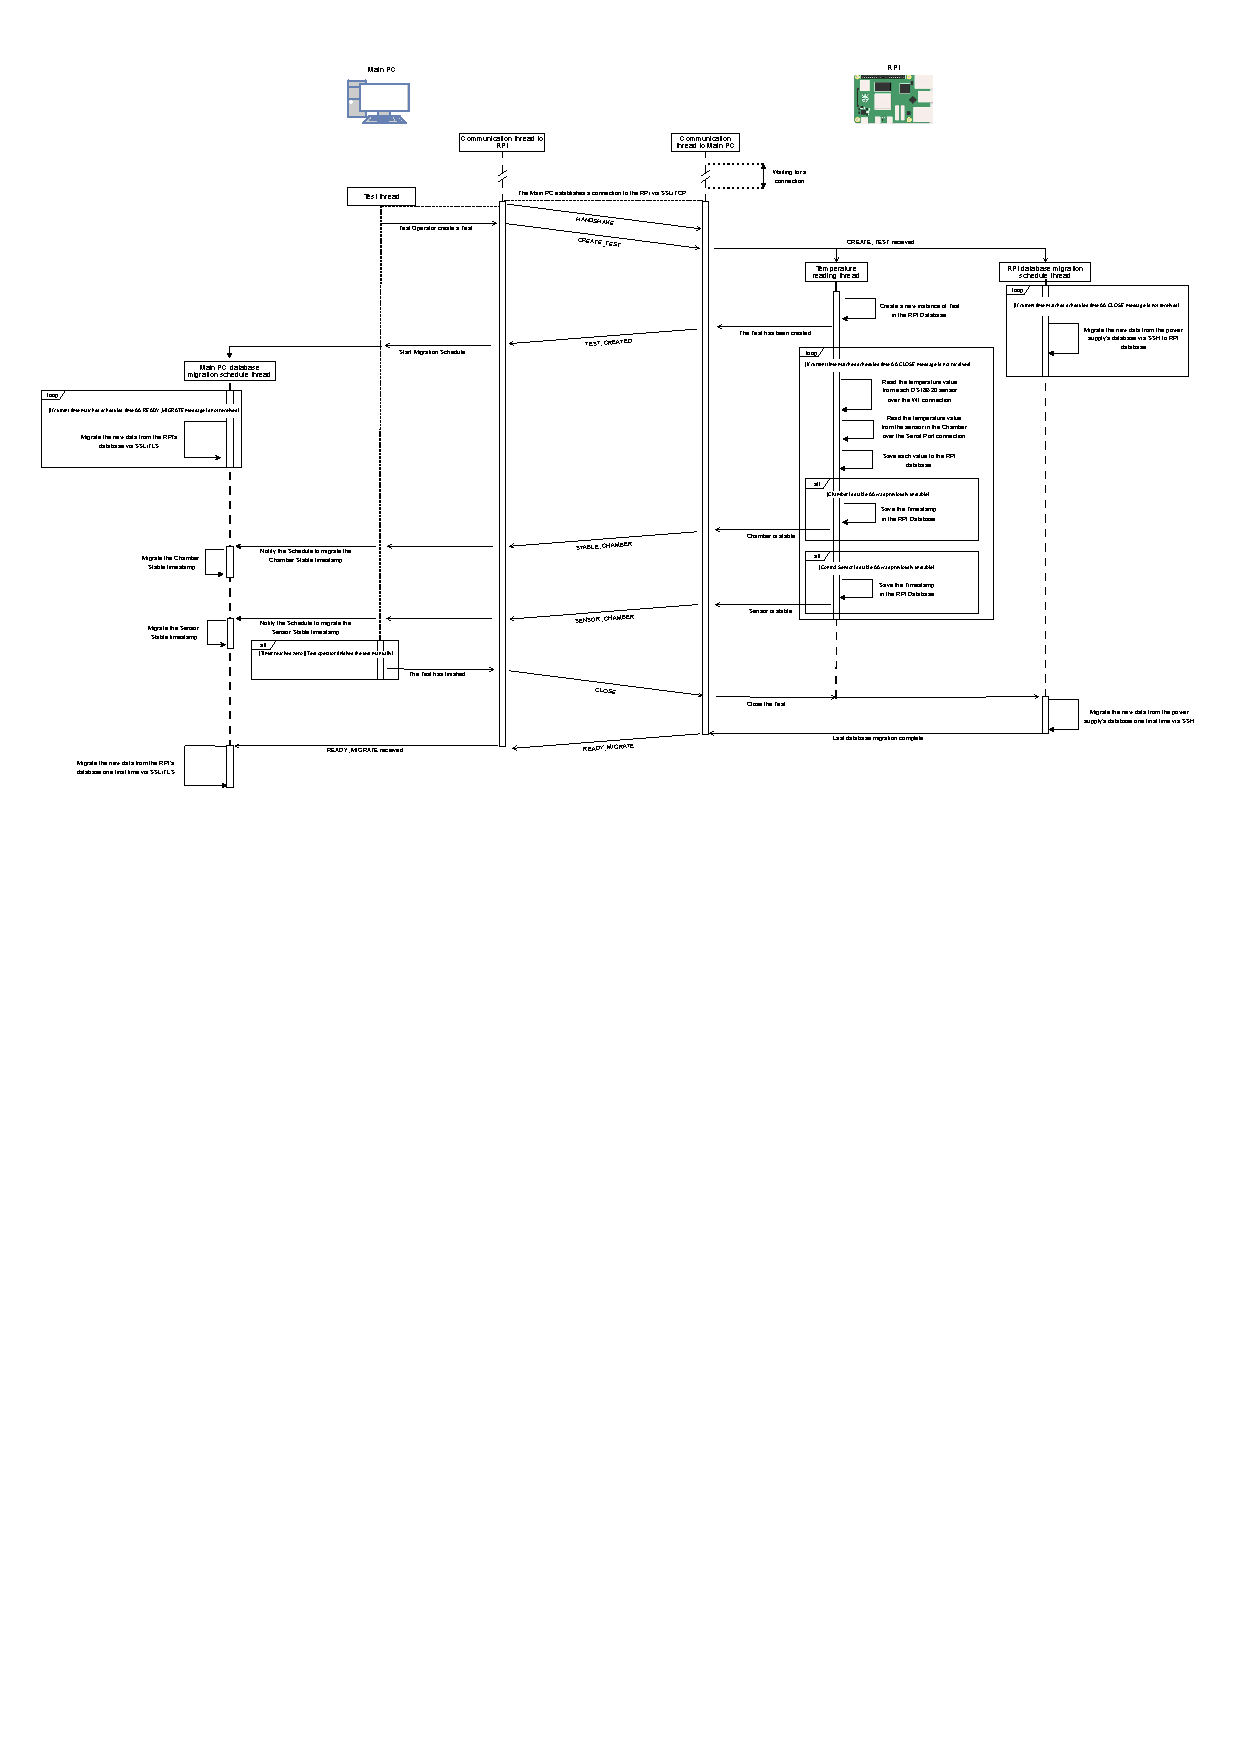
\includegraphics[width=\textwidth, clip, trim=0 16cm 0 0]{figures/communication.pdf}
    \caption{Communication protocol diagram between RPI and MainPC}
    \label{fig:diagrama_comunicacao}
\end{figure}

More information about the communication process between RPI and MainPC can be found in the general protocol documentation [DOCUMENTATION].

\subsubsection{Database}

To safeguard the integrity of temperature test data, a MySQL database was configured on the MainPC and RPI with the same schema. The schema is based on the EVSE database tables (which already existed in the laboratory) and was adapted to include the test structure. Thus, the database schema is as follows:

\begin{figure}[H]
    \centering
    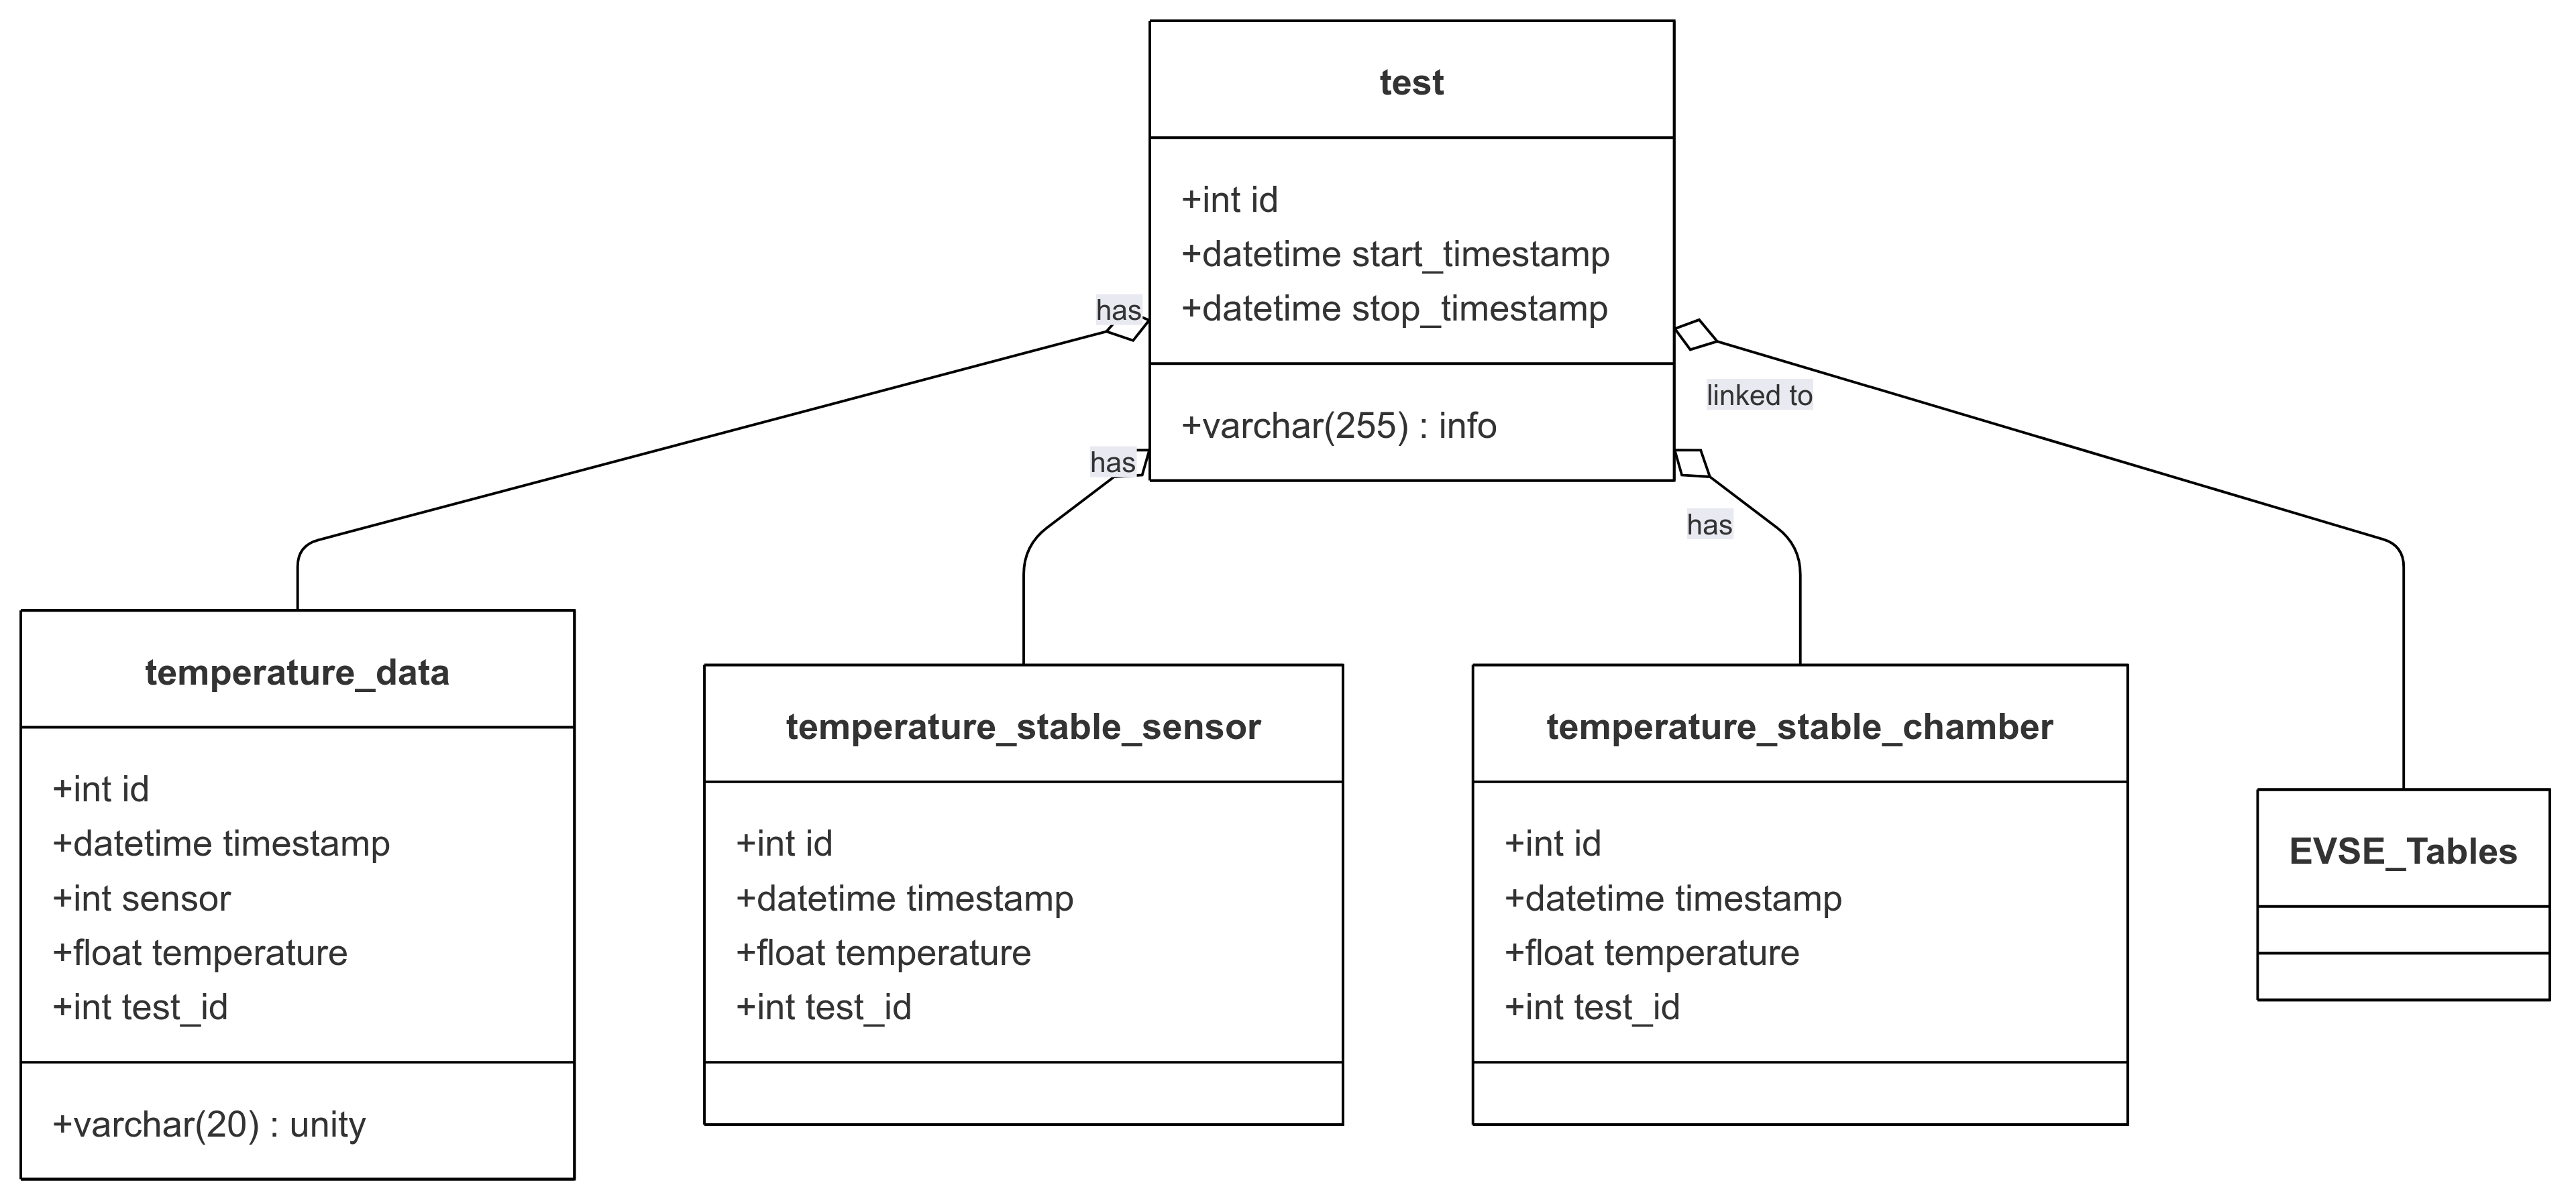
\includegraphics[width=\textwidth]{figures/class_diagram.png}
    \caption{Protocol database class diagram}
    \label{fig:class_diagram}
\end{figure}

For confidentiality reasons, the tables corresponding to EVSE data are not shown in the diagram in Figure \ref{fig:class_diagram}.
The databases are accessed through a Python library called MySQL Connector, which allows connection and manipulation of MySQL database data. The test table is the main table that stores temperature test data, while the $\mathit{temperature\_data}$ table is the table that stores temperature data obtained from DS18B20 sensors. The $\mathit{temperature\_stable\_sensor}$ and $\mathit{temperature\_stable\_chamber}$ tables are auxiliary tables that store the moment when the temperature read by the control sensor and thermal chamber sensor stabilized, respectively.

\subsubsection{Data migration and scheduling}

Scheduling is a task scheduling system that allows task execution at specific moments or at regular intervals.

Since temperature tests can last several hours, it was necessary to implement a data migration system between the three system components (RPI, MainPC, and EVSE), to allow real-time visualization of obtained data. For this, it is important to ensure synchronization between different components through communication between them. A scheduling system through threads is used to perform data migration between different system components.

The scheduling system on the RPI is responsible for obtaining data from the EVSE. The scheduling system on the MainPC is responsible for obtaining data present on the RPI (DS18B20 sensor temperature values, thermal chamber control sensor, and EVSE data).

Additionally, after the RPI notifies the MainPC that the thermal chamber control sensor and control sensor have stabilized, the MainPC scheduling system is responsible for performing the migration of this data to the MainPC database on the next trigger.

\begin{figure}[H]
    \centering
    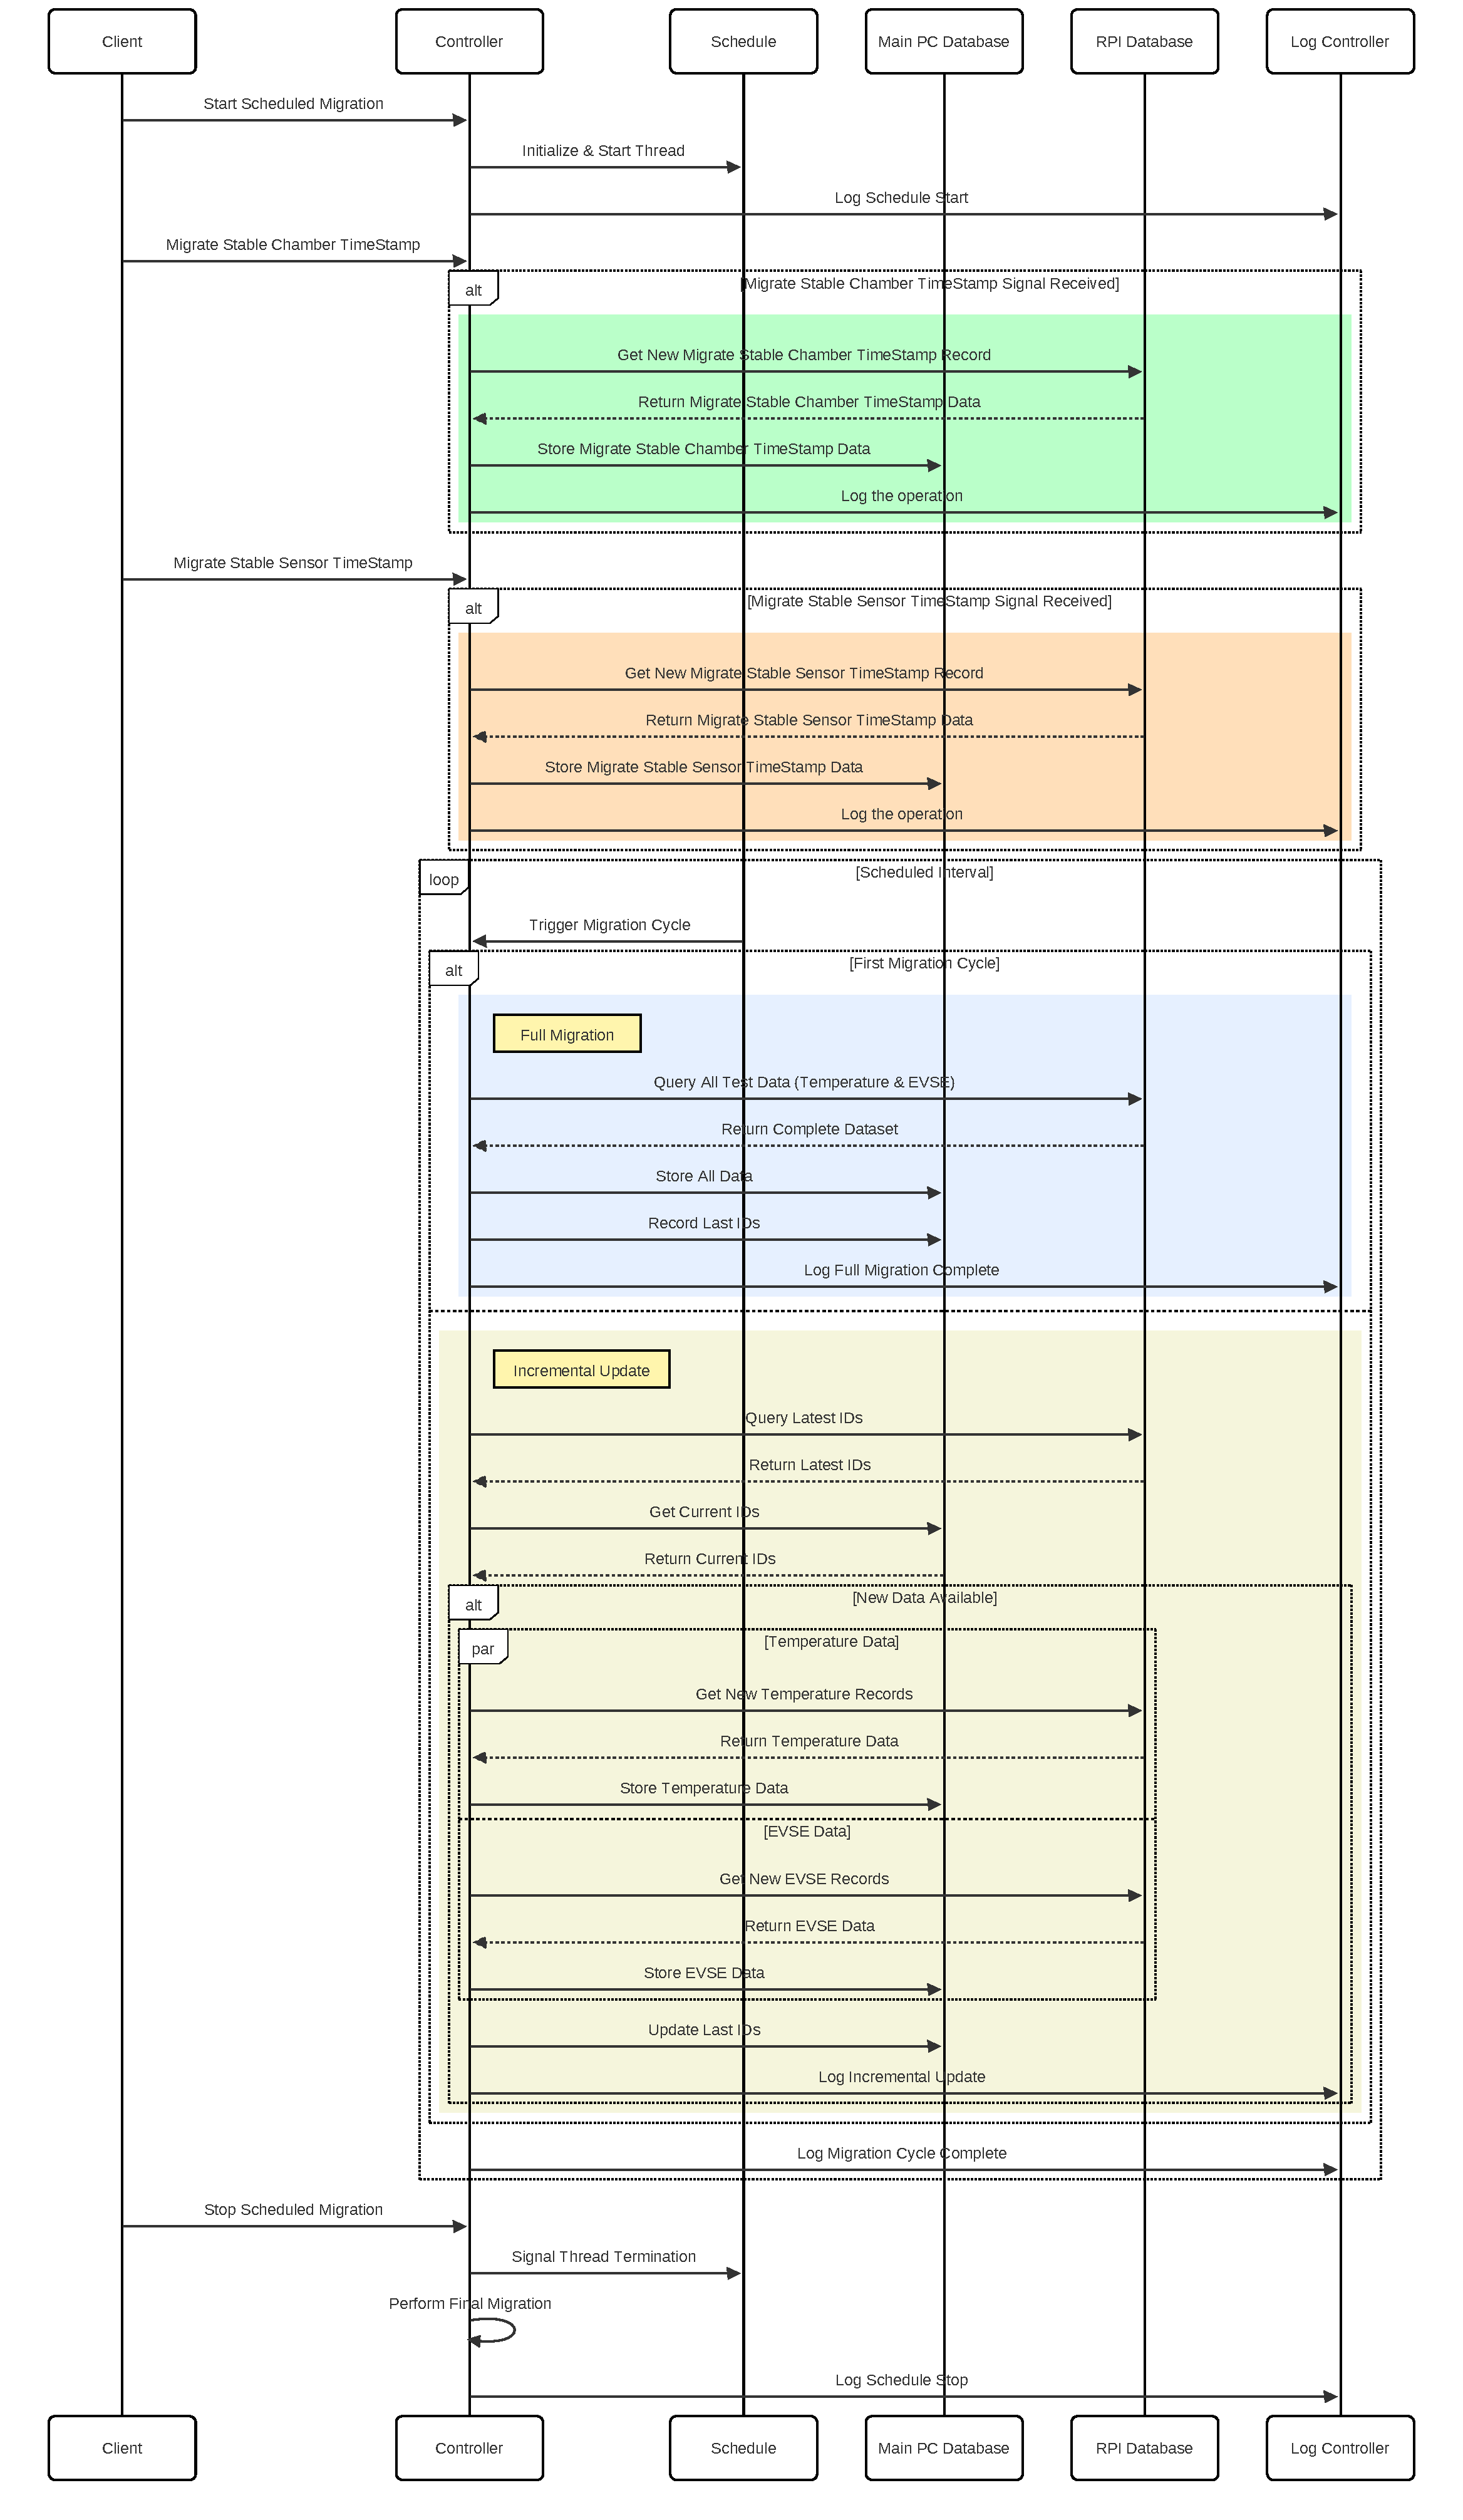
\includegraphics[scale=0.10]{figures/scheduling_1.pdf}
    \caption{MainPC scheduling system sequence diagram}
    \label{fig:scheduling_1}
\end{figure}

\begin{figure}[H]
    \centering
    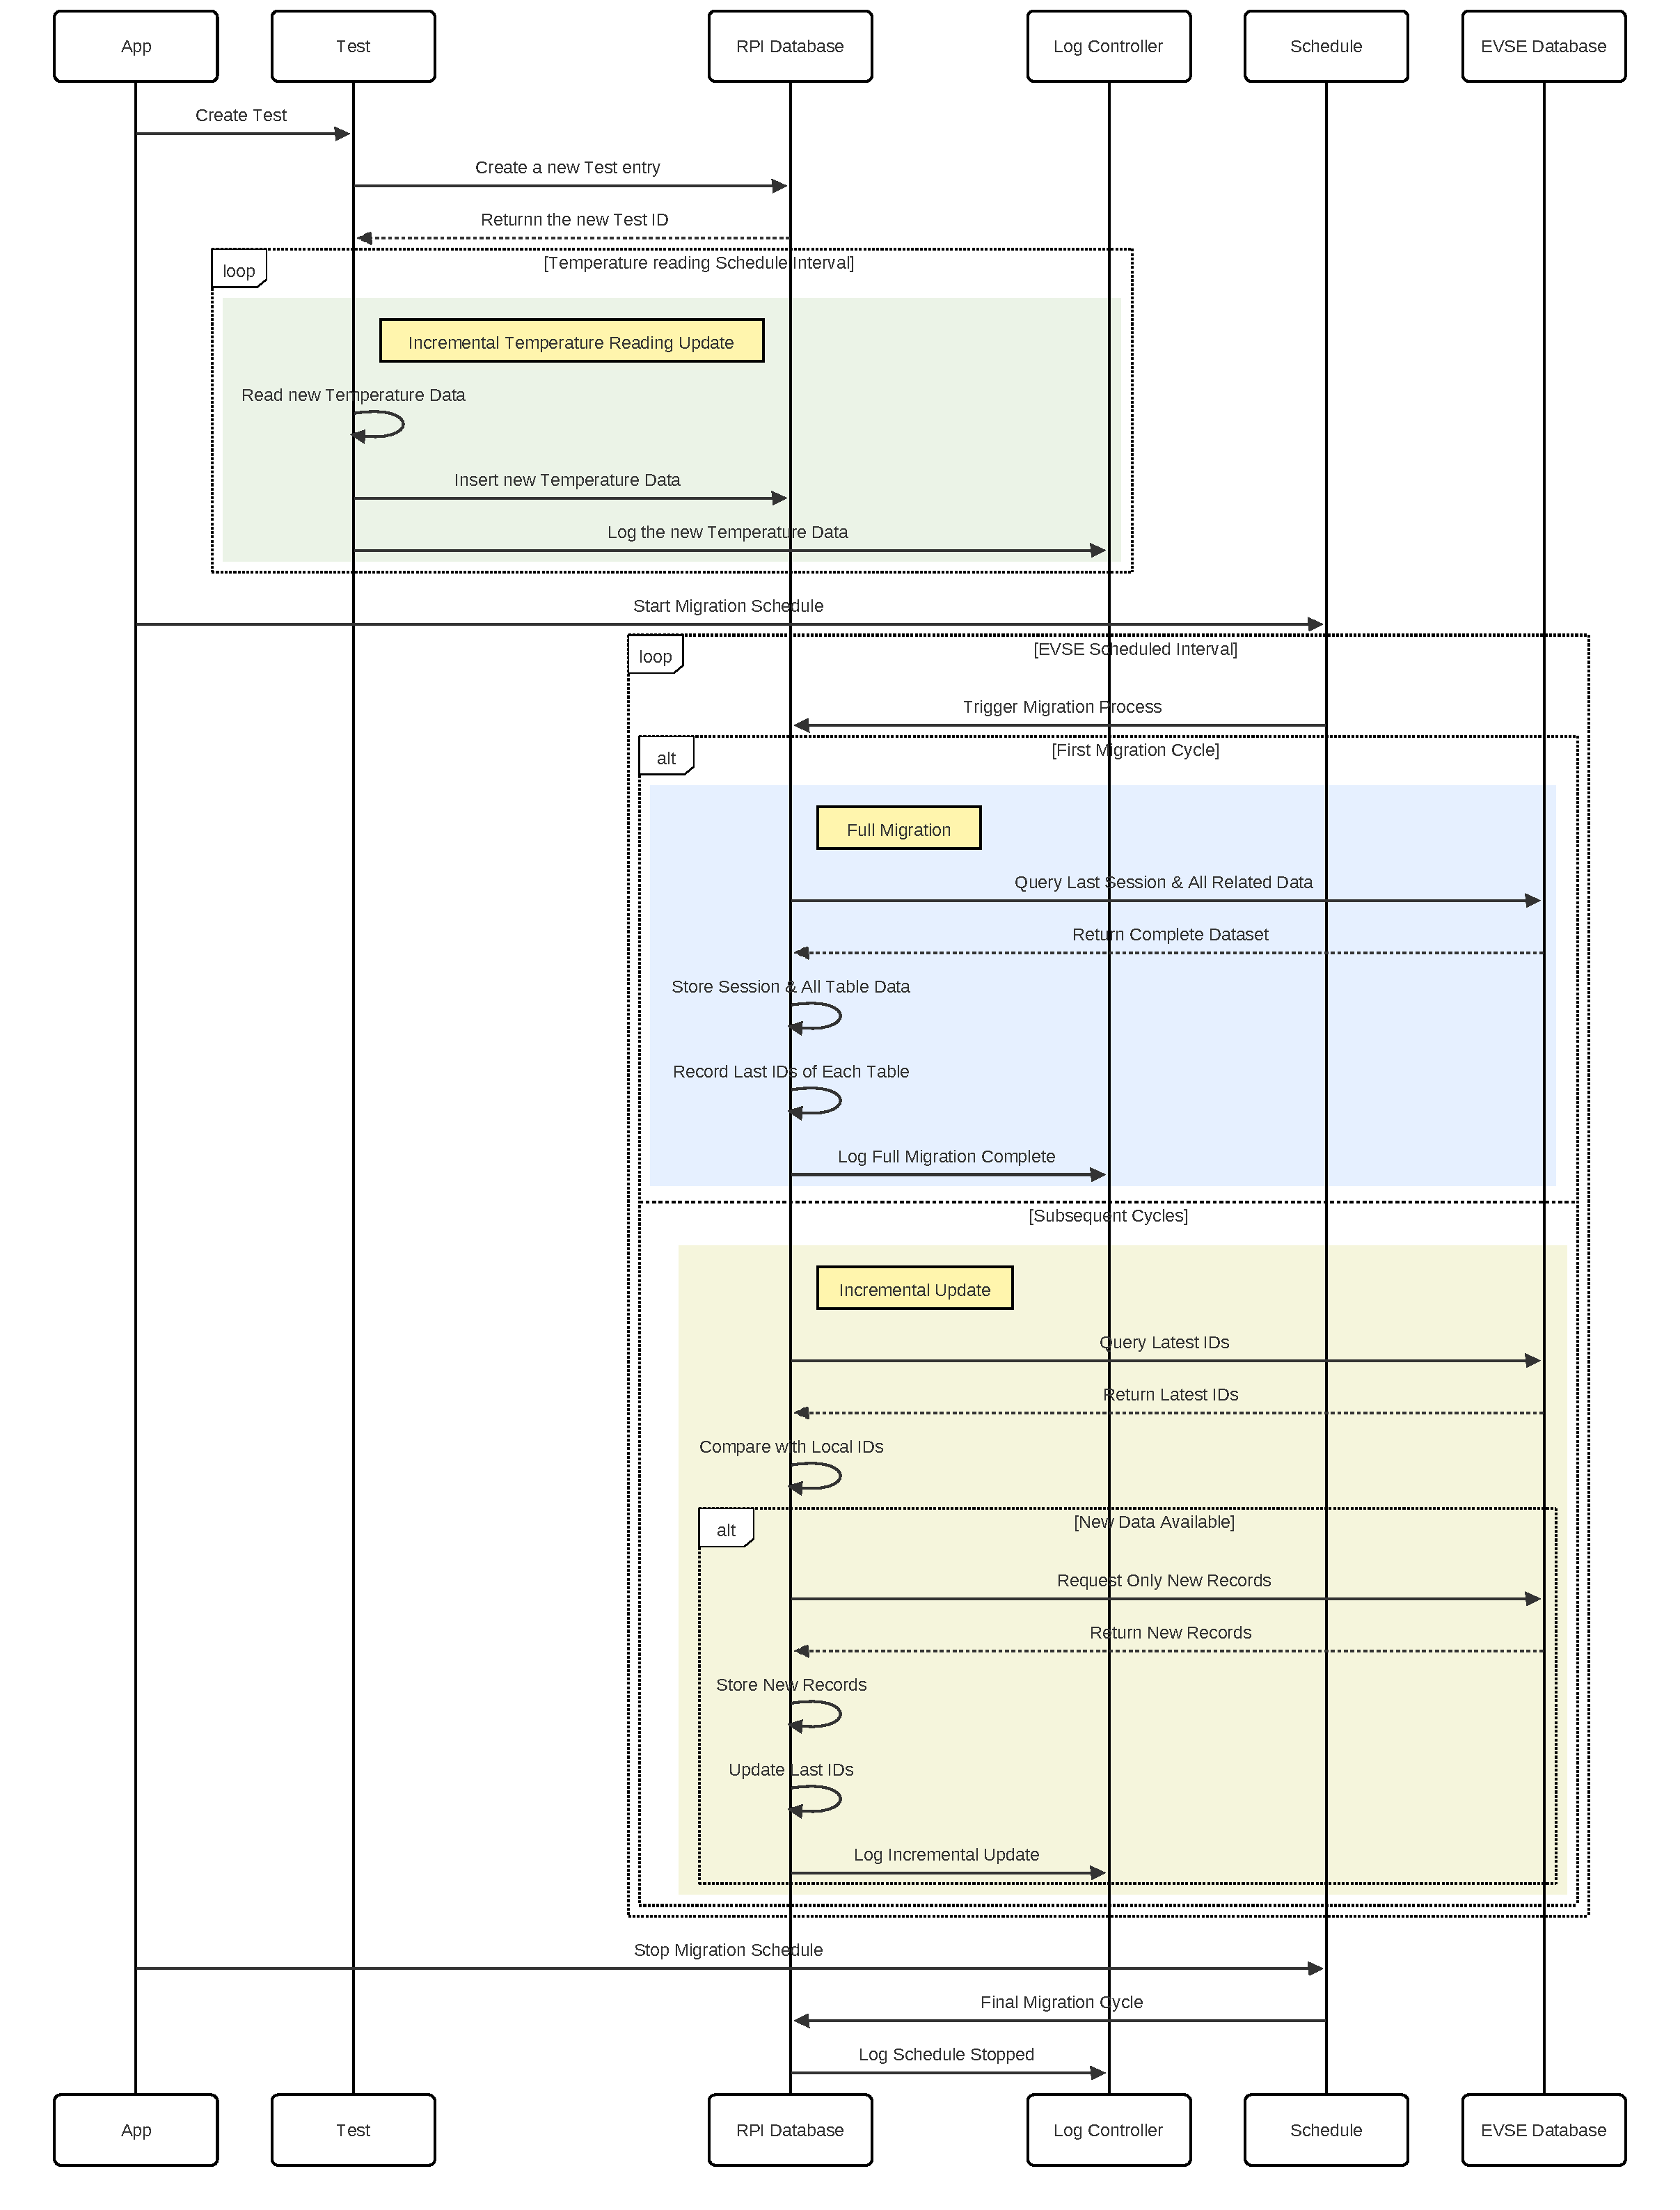
\includegraphics[scale=0.10]{figures/scheduling_2.pdf}
    \caption{RPI scheduling system sequence diagram}
    \label{fig:scheduling_2}
\end{figure}

\subsubsection{Dashboard}
A dashboard is a graphical interface that allows visualizing data in an interactive and customized way. The main objective of the dashboard is to allow the user to visualize temperature test data obtained in real time and charger data in real time.

Grafana not only allows real-time graphical visualization of obtained data, but also automatic creation of annotations to show the moments when temperature stabilized (both for the thermal chamber control sensor and EVSE control sensor).

Additionally, it is possible to insert the theoretical power value of the charger to calculate the efficiency of electric car charging over time, allowing more detailed analysis of charging performance.

Another important factor is the easy switching of test visualization, allowing the user to select the test they want to visualize and analyze the obtained data. 

\begin{figure}[H]
    \centering
    \begin{minipage}{0.8\textwidth}
        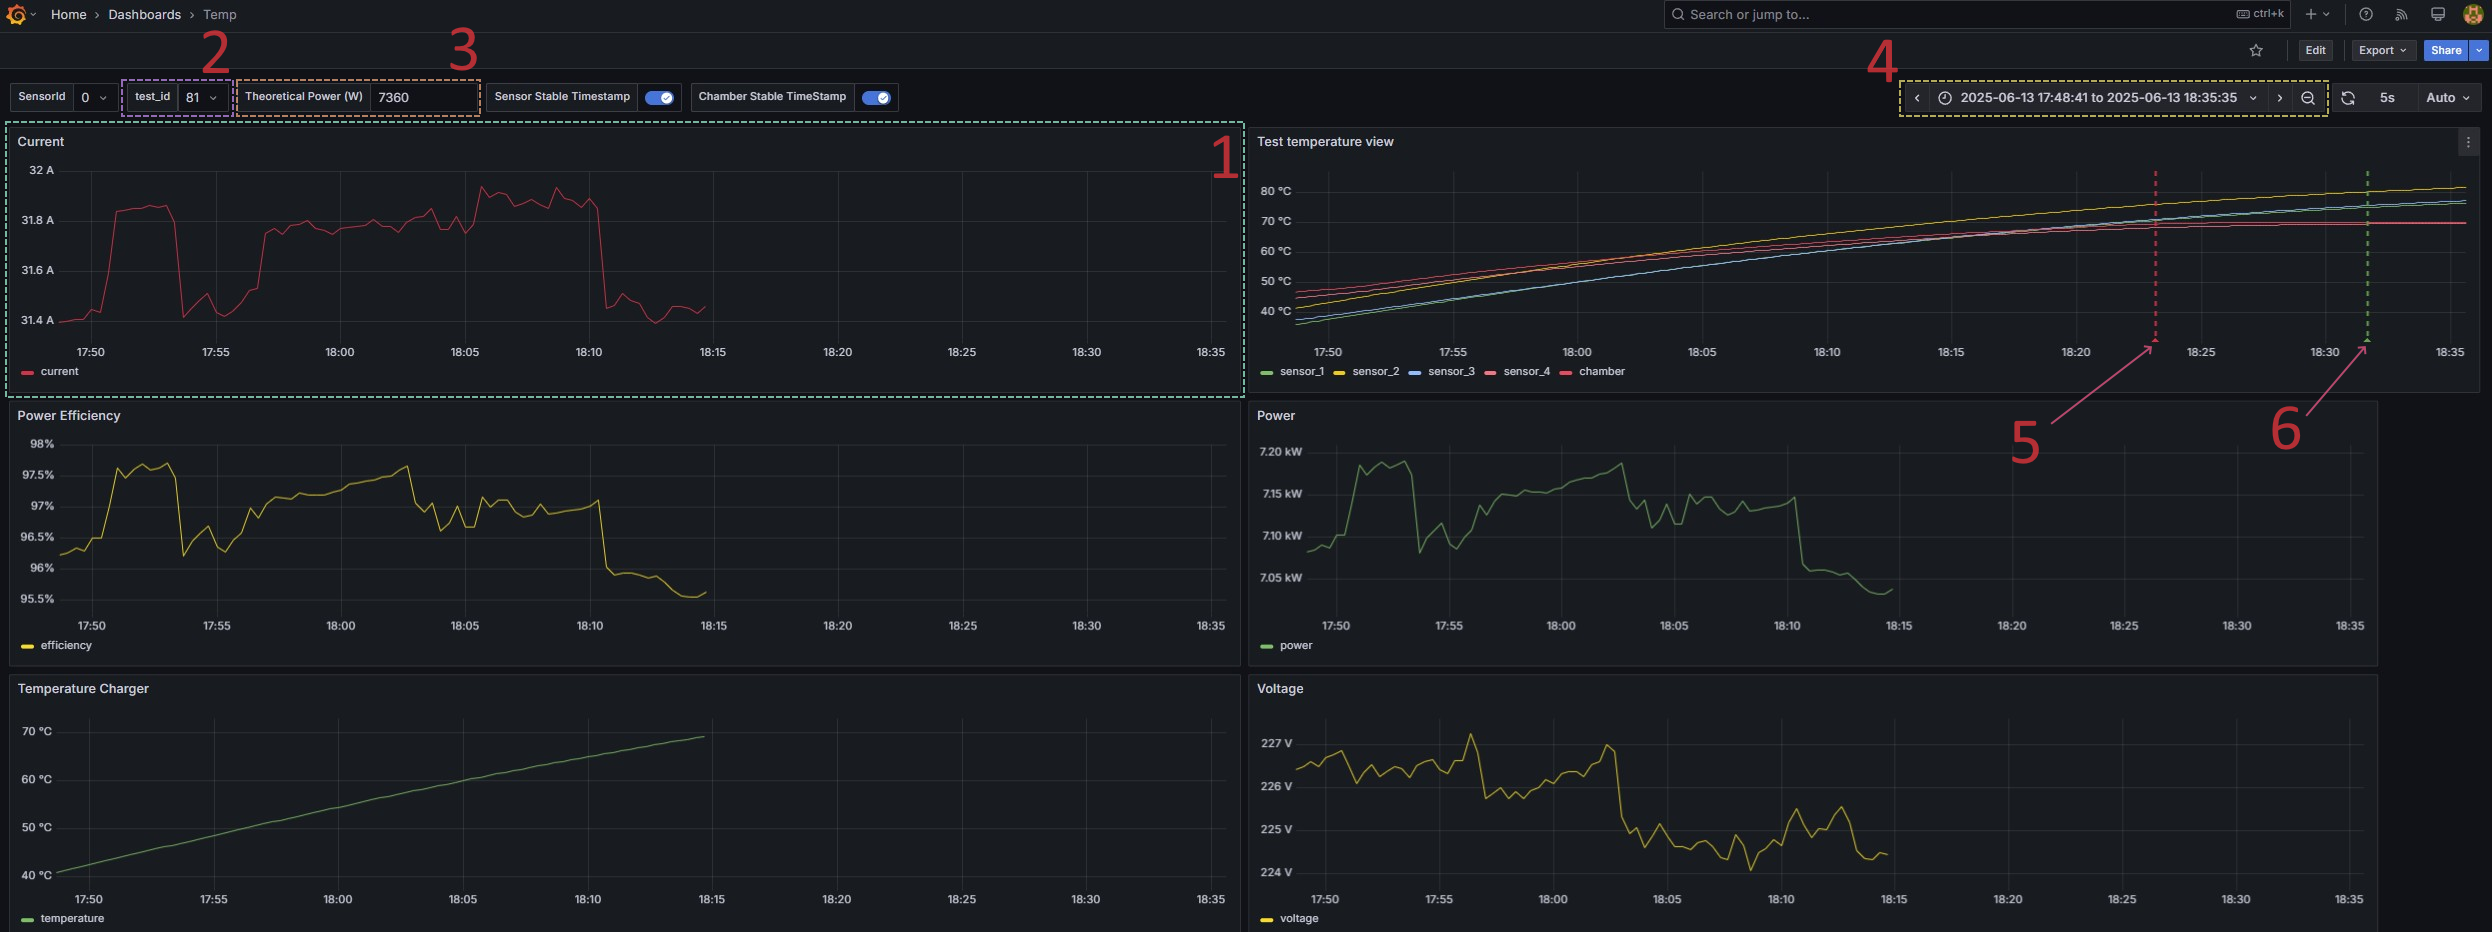
\includegraphics[width=\linewidth]{figures/dashboard.png}
    \end{minipage}
    \caption{Test data visualization dashboard}
    \label{fig:dashboard}
    
    \vspace{0.5em}
    \begin{minipage}{0.95\textwidth}
        \small
        \textbf{Legend:}
        \begin{enumerate}
            \item Example graph for visualizing test data obtained
            \item Test selection dropdown (via $test\_id$)
            \item Input box for theoretical charger power value
            \item Time interval selection for data visualization
            \item Automatic annotation of thermal chamber sensor temperature stabilization
            \item Automatic annotation of control sensor temperature stabilization
        \end{enumerate}
    \end{minipage}
\end{figure}

\subsubsection{Installation and configuration}
One of the tasks developed during the internship was system bootstrapping, to allow its rapid installation and configuration. For RPI component installation, Ansible was used while for MainPC component installation, a dockerfile with devcontainer integration was used (more information in [DOCUMENTATION]).

After initial setup and system configuration, the different hardware components must be properly connected and positioned. In the following figures, their installation can be seen (more information in [DOCUMENTATION]):

\begin{figure}[H]
    \centering
    \begin{minipage}{0.6\textwidth}
        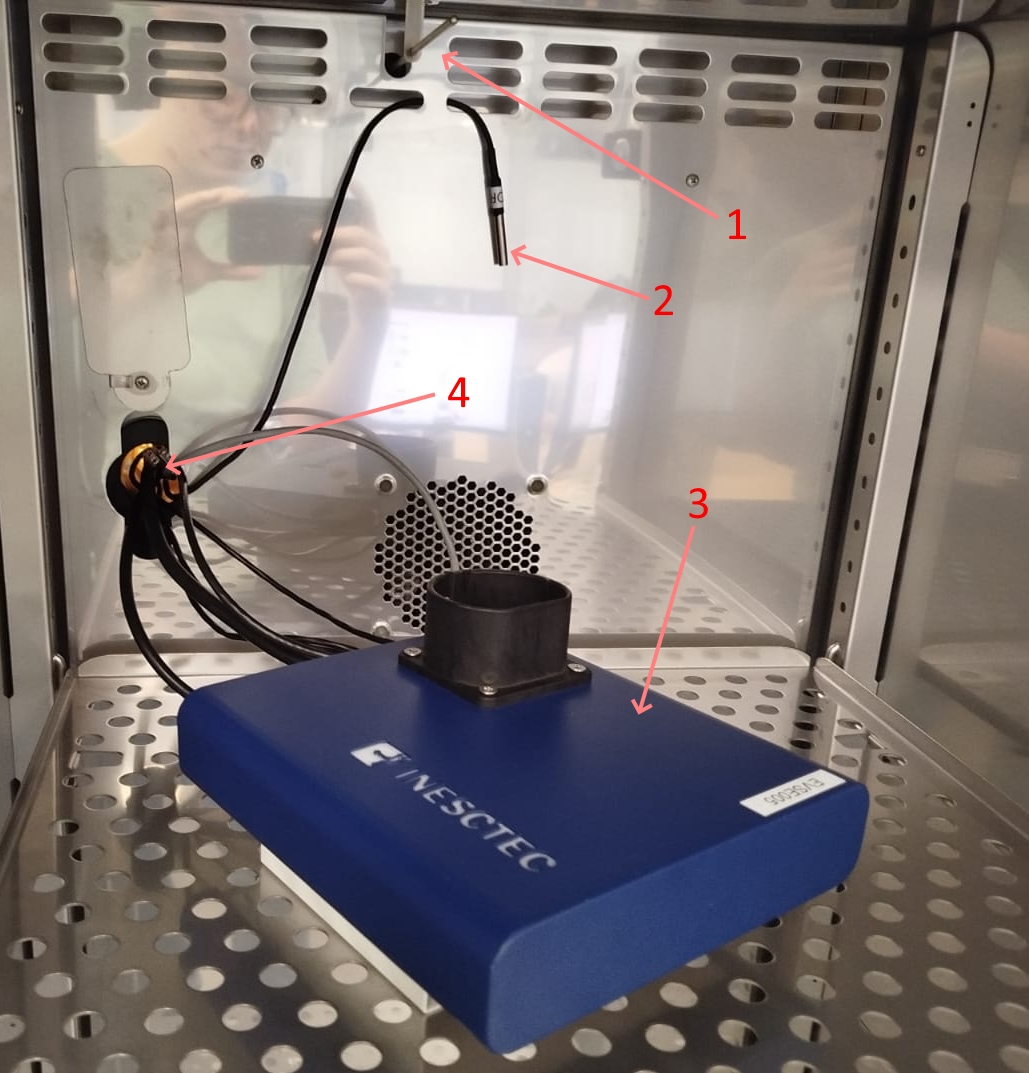
\includegraphics[width=\linewidth]{figures/inst_inside_1.png}
    \end{minipage}%
    \hfill
    \begin{minipage}{0.35\textwidth}
        \small
        \textbf{Legend:}
        \begin{enumerate}
            \item Thermal chamber sensor
            \item DS18B20 thermal chamber temperature control sensor
            \item EVSE
            \item Exit to the exterior of the thermal chamber
        \end{enumerate}
    \end{minipage}
    \caption{Image of EVSE inside the thermal chamber}
    \label{fig:inst_inside_1}
\end{figure}

\begin{figure}[H]
    \centering
    \begin{minipage}{0.6\textwidth}
        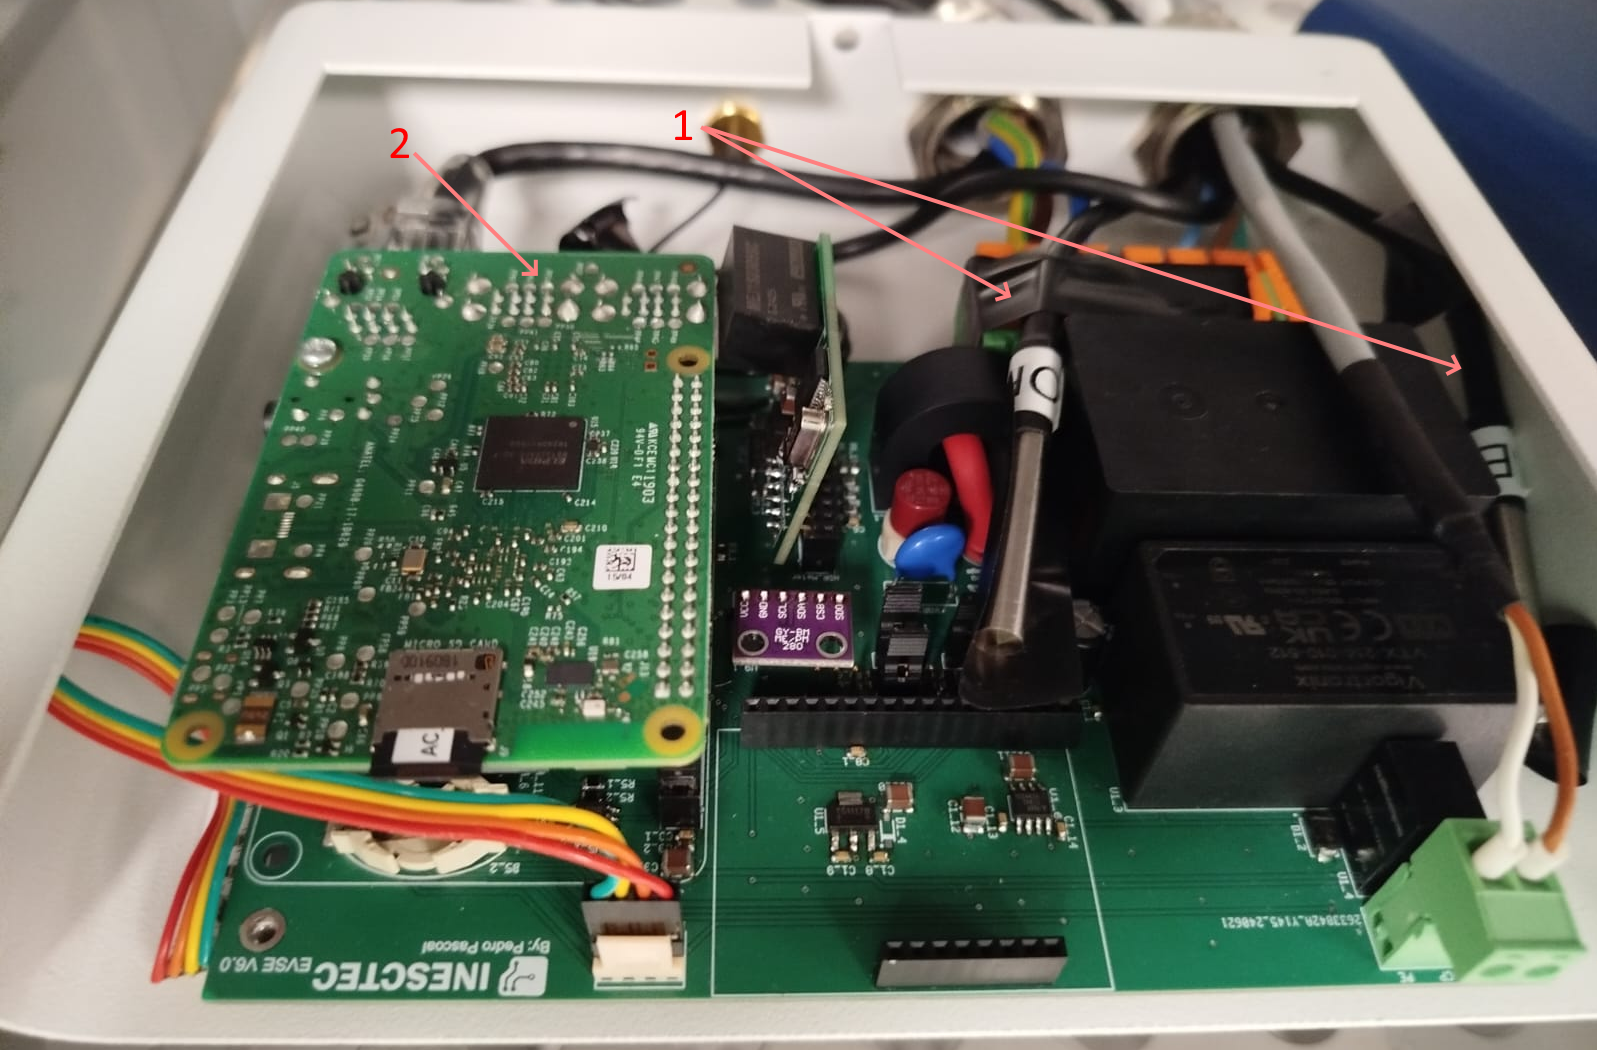
\includegraphics[width=\linewidth]{figures/inst_inside_2.png}
    \end{minipage}%
    \hfill
    \begin{minipage}{0.35\textwidth}
        \small
        \textbf{Legend:}
        \begin{enumerate}
            \item DS18B20 sensors positioned inside the EVSE
            \item EVSE Raspberry
        \end{enumerate}
    \end{minipage}
    \caption{Positioning of DS18B20 sensors inside the EVSE}
    \label{fig:inst_inside_2}
\end{figure}

\begin{figure}[H]
    \centering
    \begin{minipage}{0.6\textwidth}
        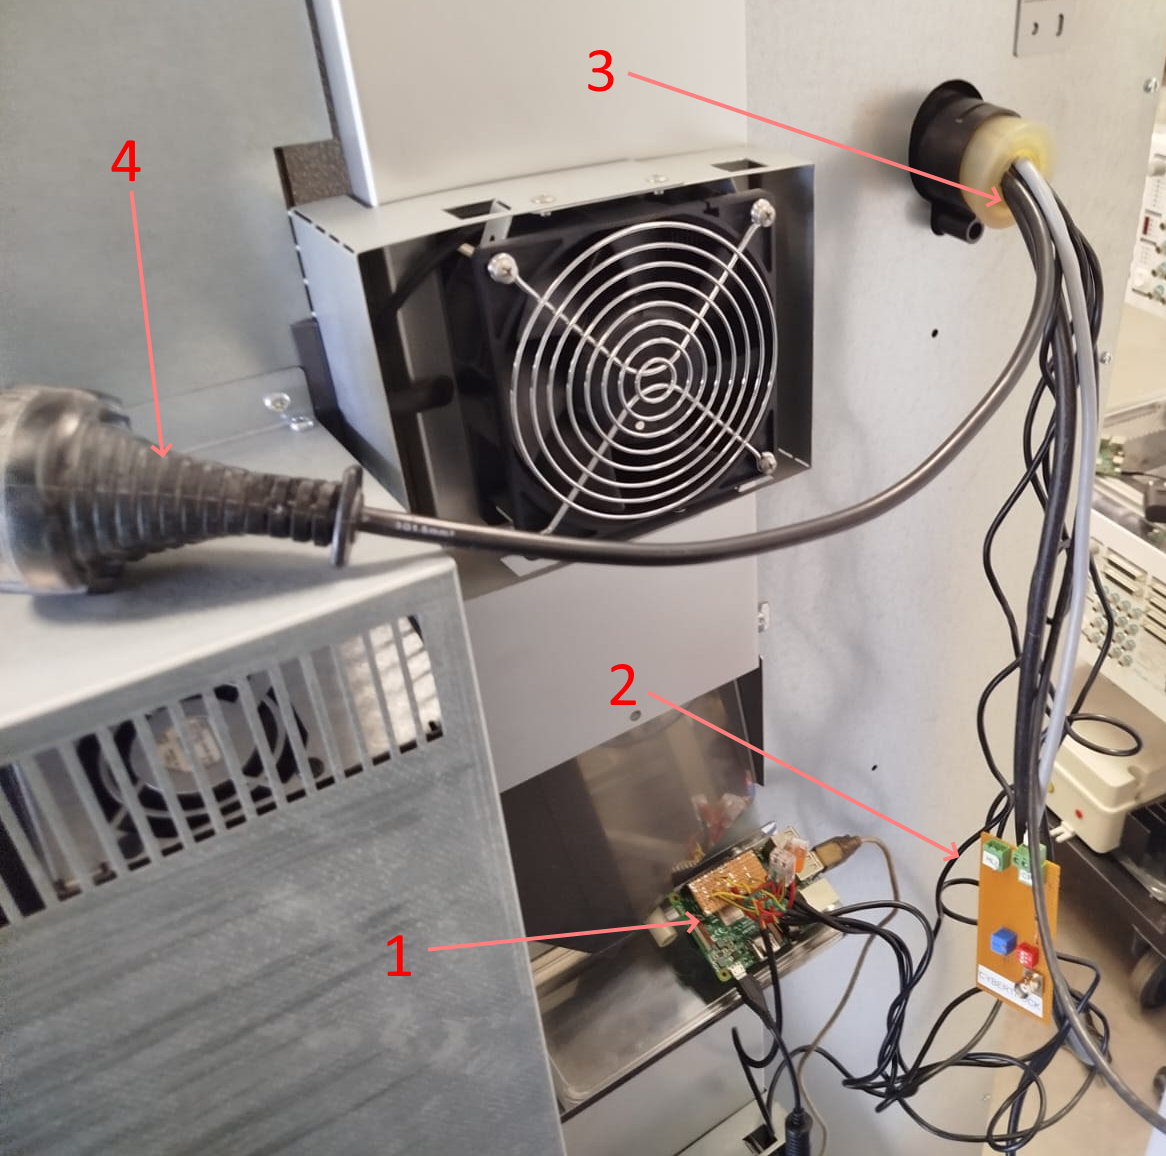
\includegraphics[width=\linewidth]{figures/inst_inside_3.png}
    \end{minipage}%
    \hfill
    \begin{minipage}{0.35\textwidth}
        \small
        \textbf{Legend:}
        \begin{enumerate}
            \item Test control RPI
            \item ... TODO
            \item Entry to the interior of the thermal chamber
            \item ... TODO
        \end{enumerate}
    \end{minipage}
    \caption{External rear part of the thermal chamber}
    \label{fig:inst_inside_3}
\end{figure}

\begin{figure}[H]
    \centering
    \begin{minipage}{0.6\textwidth}
        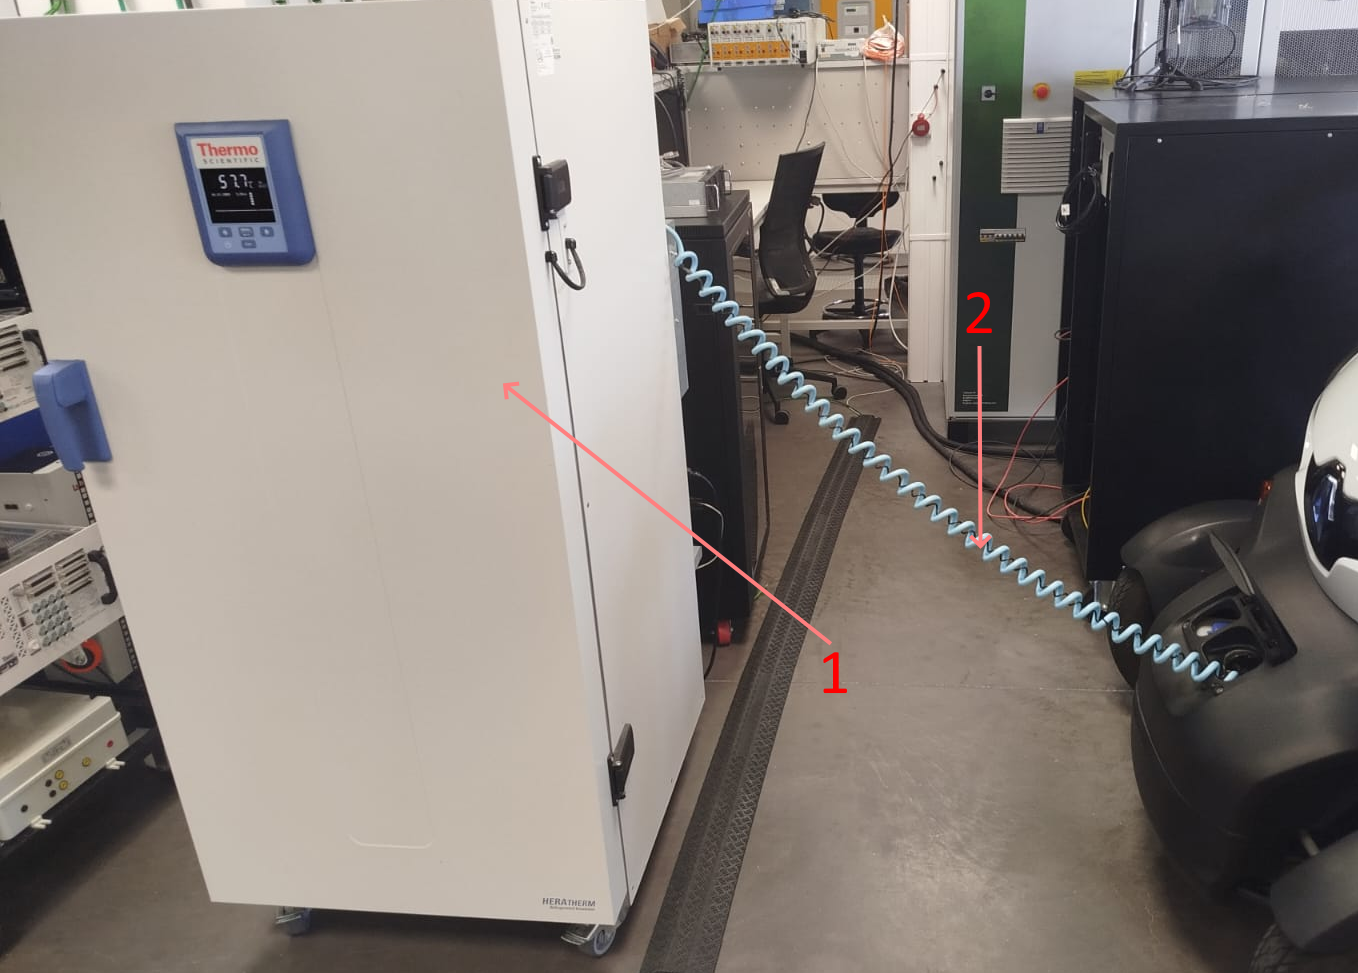
\includegraphics[width=\linewidth]{figures/inst_inside_4.png}
    \end{minipage}%
    \hfill
    \begin{minipage}{0.35\textwidth}
        \small
        \textbf{Legend:}
        \begin{enumerate}
            \item IMP 400 thermal chamber
            \item Car charging cable
        \end{enumerate}
    \end{minipage}
    \caption{External rear part of the thermal chamber}
    \label{fig:inst_inside_4}
\end{figure}

\subsection{Validation}

For protocol validation, several tests were carried out throughout the internship. The most relevant tests performed were the following:
\begin{itemize}
    \item DS18B20 sensor precision and accuracy: Place DS18B20 sensors inside the thermal chamber and verify if the values read by the sensors are consistent with the thermal chamber temperature (several iterations were performed with different chamber temperatures);
    \item Scheduling: Verify if the scheduling system is working correctly with all system components (MainPC, RPI, and EVSE). For this, DS18B20 sensors were placed in the thermal chamber while the EVSE was outside the chamber sending data without any charging taking place;
    \item Logistics: Verify the arrangement of three DS18B20 sensors inside the EVSE inside the thermal chamber. It also served to verify our hypothesis that the charger would be at a lower temperature than the thermal chamber while the thermal chamber temperature was not stabilized (increasing temperature, for example), but that eventually the charger would reach a temperature higher than the thermal chamber;
    \item Test with an electric vehicle: To validate the protocol under real conditions, a test was performed with different electric vehicles that require different charging powers. The results obtained not only validated the protocol, but also allowed verifying the efficiency of electric car charging over time.
\end{itemize}

The results obtained from tests performed under real conditions revealed that the EVSE charger at high temperatures (above 60°C) can maintain charging efficiency above 95\% (which is considered acceptable for electric vehicle charging).

(TODO add more information about the tests performed and results obtained)